\documentclass[tikz,border=8pt]{standalone}
% Shared look for every TikZ diagram. Load with \input{../../tools/tikz-style.tex}
\usepackage[T1]{fontenc}
\usepackage{lmodern}
\renewcommand{\sfdefault}{lmr}  % diagrams use the same serif as the text
\usetikzlibrary{arrows.meta, positioning, shapes.geometric, calc, fit, backgrounds}
\definecolor{cblue}{HTML}{4C78A8}
\definecolor{corange}{HTML}{F58518}
\definecolor{cgreen}{HTML}{54A24B}
\definecolor{cred}{HTML}{E45756}
\definecolor{cpurple}{HTML}{B279A2}
\definecolor{cgrey}{HTML}{6B6B6B}
\tikzset{
  every picture/.style={font=\sffamily, line width=1.2pt},
  box/.style={draw=#1, fill=#1!12, rounded corners=4pt, align=center, inner sep=7pt, minimum height=1.1cm},
  box/.default=cgrey,
  arrow/.style={-{Stealth[length=3mm]}, draw=cgrey, line width=1.4pt},
  title/.style={font=\sffamily\bfseries\Large},
  note/.style={font=\sffamily\small, text=cgrey, align=center},
}
\AtBeginDocument{\hyphenpenalty=10000 \exhyphenpenalty=10000}

\begin{document}
\begin{tikzpicture}
  \node[box=cgrey, font=\sffamily\bfseries\large, minimum width=4.6cm] (fs) at (4.2,0) {Feature scaling};
  \node[box=cblue, font=\sffamily\bfseries, text width=3.6cm, minimum height=1.4cm] (st) at (0,-2.2) {Standardization\\[-1pt]\normalfont\small (this Note)};
  \node[box=cgrey, fill=white, font=\sffamily\bfseries, text width=3.6cm, minimum height=1.4cm, dashed] (no) at (8.4,-2.2) {Normalization\\[-1pt]\normalfont\small (next Note)};
  \draw[arrow] (fs.south) -- (st.north);
  \draw[arrow] (fs.south) -- (no.north);
  % the two steps of standardization
  \node[box=cgreen, text width=3.4cm, anchor=north] (s1) at (-2.1,-4.0) {\textbf{1. Mean centring}\\[2pt] subtract the mean\\[1pt] \small mean becomes 0};
  \node[box=corange, text width=3.4cm, anchor=north] (s2) at (2.1,-4.0) {\textbf{2. Scaling}\\[2pt] divide by the std\\[1pt] \small std becomes 1};
  \draw[arrow] (st.south) -- (s1.north);
  \draw[arrow] (st.south) -- (s2.north);
  \node[font=\sffamily\Large, anchor=north] at (0,-6.6) {$z = \dfrac{x - \text{mean}}{\text{std}}$};
  \node[note, text=black, text width=4.2cm, anchor=north] at (8.4,-4.0) {min-max scaling and others:\\ squeeze every column\\ into a fixed range};
\end{tikzpicture}
\end{document}
